\message{ !name(showv2.tex)}\documentclass[mode=present,style=simple]{powerdot}

%\usepackage{simpsons}
\usepackage[utf8]{inputenc}
\usepackage{natbib}
\usepackage{graphicx}
\usepackage{multirow}
\usepackage{bbding}
\usepackage{manfnt}
\usepackage{fourier}
\usepackage[labelfont=bf,textfont=sl,tableposition=top,scriptsize]{caption}
\usepackage{amsmath,amsfonts,amssymb,amsthm}
\usepackage{mathrsfs}

\theoremstyle{plain}% default
\newtheorem{thm}{Theorem}%[section]
\newtheorem{lem}{Lemma}
\newtheorem{prop} {Proposition}
\newtheorem{cor}{Corollary}
\theoremstyle{definition}
\newtheorem{defn}{Definition}%[section]
\newtheorem{conj}{Conjecture}%[section]
\newtheorem{exmp}{Example}%[section]
\theoremstyle{remark}
\newtheorem*{rem}{Remark}
\newtheorem{case}{Case}

\newcommand{\advice}[1]{\HandPencilLeft{} \emph{#1}}


\title{Statistical modelling of spatial extremes using the SpatialExtremes package}
\author{M. Ribatet}
\date{University of Montpellier}
% \date{
%   \begin{center}
%     $^\dag$ Laboratoire de Mathématiques et Application, Université de
%     Poitiers\\
%     $^\ddag$ Institut de Mathématiques et de Modélisation, Université
%     Montpellier 2
%   \end{center}
% }


\pdsetup{
  lf={The \texttt{SpatialExtremes} package},
  rf={Mathieu Ribatet},
  logohook=tr,
  logopos={.99\slidewidth,.99\slideheight},
  logocmd={},%\includegraphics[height=.08\slideheight]{Figures/logoI3M}},
  counters={thm,lem,prop,cor,defn,conj,exmp,case,figure},
}

\begin{document}

\message{ !name(showv2.tex) !offset(76) }
\section{1. Data and descriptive analysis}

\begin{slide}[toc=Data format,method=direct]{Required data}
  Before introducing more advanced stuff, let's talk about data
  format. It is pretty simple
  \begin{description}
  \item[Observations] A numeric matrix such that \textcolor{blue}{each
      row is one realization of the spatial field}---or if you prefer
    one column per site;
  \item[Coordinates] A numeric matrix such that \textcolor{blue}{each
      row is the coordinates of one site}---or if you prefer the first
    column is for instance the longitude of all sites, the second one
    latitude, \ldots
  \end{description}
{\tiny
  \begin{minipage}[l]{.49\linewidth}
\begin{verbatim}
> data
       Valkenburg  Ijmuiden  De Kooy  ...
 1971         278        NA      360  ...
 1972         334        NA      376  ...
 1973         376        NA      365  ...
 1974         314        NA      304  ...
 1975         278        NA      278  ...
 1976         350        NA      345  ...
 1977         324        NA      298  ...
 1978         298        NA      329  ...
 1979         252        NA      298  ...
 ...
\end{verbatim}%
  \end{minipage}%
  \begin{minipage}[r]{.49\linewidth}
\begin{verbatim}
> coord
                        lon        lat
 Valkenburg           4.419     52.165
 Ijmuiden             4.575     52.463
 De Kooy              4.785     52.924
 Schiphol             4.774     52.301
 Vlieland             4.942     53.255
 Berkhout             4.979     52.644
 Hoorn                5.346     53.393
 De Bilt              5.177     52.101
 ...
\end{verbatim}
  \end{minipage}
}
\end{slide}

\begin{slide}[toc=,method=direct]{Additional covariates}
  In addition to the storage of observations and coordinates, you
  might want to use additional covariates. The latter can be of two
  types
  \begin{description}
  \item[Spatial] A numeric matrix such that \textcolor{blue}{each
      column corresponds to one spatial covariate} such as elevation,
    urban/rural, \ldots
  \item[Temporal] A numeric matrix such that \textcolor{blue}{each
      column corresponds to one temporal covariate} such as time,
    annual mean temperature, \ldots
  \end{description}
{\tiny
  \begin{minipage}[l]{.49\linewidth}
\begin{verbatim}
> spat.cov
                     alt
 Valkenburg         -0.2
 Ijmuiden            4.4
 De Kooy             0.5
 Schiphol           -4.4
 Vlieland            0.9
 Berkhout           -2.5
 Hoorn               0.5
 De Bilt             2.0
 ...
\end{verbatim}
  \end{minipage}%
  \begin{minipage}[r]{.49\linewidth}
\begin{verbatim}
> temp.cov
               nao
 1971         1.87
 1972         1.57
 1973        -0.20
 1974        -0.95
 1975        -0.46
 1976         2.34
 1977        -0.49
 1978         0.70
 1979         1.11
 ...
\end{verbatim}
  \end{minipage}
}

\advice{It is always a good idea to name your columns and rows.}
\end{slide}

\begin{slide}[toc=First look]{Inspecting data}
  \begin{itemize}
  \item As usual, you first have to \textcolor{blue}{scrutinize your
      data} (weird values, encoding of missing values, check out
    factors, \ldots). But you're used to that, aren't you?
  \item We focus on extremes, so you may wonder
    \begin{itemize}
    \item are my data \textcolor{blue}{extremes}, i.e., block maxima?
    \item is my \textcolor{blue}{block size} relevant?
    \item what about \textcolor{blue}{seasonality}? Refine the block
      or use temporal covariate?
    \end{itemize}
  \item You might want to \textcolor{blue}{check that the generalized
      extreme value family is sensible for your data}---the
    \texttt{evd} package + a few lines of code will do the job for you
    (homework)
  \item This will generally be OK, but now you have to go a bit
    further by analyzing
    \begin{itemize}
    \item the spatial dependence ;
    \item and the presence / absence of any spatial trends.
    \end{itemize}
  \end{itemize}
\end{slide}

\begin{slide}{Spatial dependence}
  \begin{itemize}
  \item Essentially you want to check if your data exhibit any
    (spatial) dependence. If not why would you bother with spatial
    models?
  \item The most convenient way to do this is through the
    \textcolor{blue}{$F$-madogram} and its connection with the
    \textcolor{blue}{extremal coefficient}:
    \begin{equation*}
      \nu_F(h) = \frac{1}{2} \mathbb{E} [| F\{Z(o)\} - F\{Z(h)\}| ],
      \qquad \theta(h) = \frac{1 + 2 \nu_F(h)}{1 - 2 \nu_F(h)}.
    \end{equation*}
  \item The \texttt{fmadogram} function will estimate (empirically)
    the pairwise extremal coefficent from the $F$--madogram.
  \end{itemize}

  \fcolorbox{blue}{white}{
    
    \Homer
    \begin{equation*}
      \theta(h) = - z \log \Pr\{Z(s) \leq z, Z(s + h) \leq z\}
    \end{equation*}
    and that $1 \leq \theta(h) \leq 2$ with complete dependence iff
    $\theta(h) = 1$ and independence iff $\theta(h) = 2$.
  }
\end{slide}

\begin{wideslide}[toc=]{The \texttt{fmadogram} function}
  \vspace{-1.5em}
  \begin{itemize}
  \item Run the file \texttt{fmadogram.R}. You should get the figure
    below.
  \item<2-> You can also use a binned version with \texttt{n.bins =
      300}\ldots
  \end{itemize}
  \begin{figure}
    \centering
    \onslide*{1}{\includegraphics[width=.75\textwidth]{Figures/fmadogram}}
    \onslide*{2-}{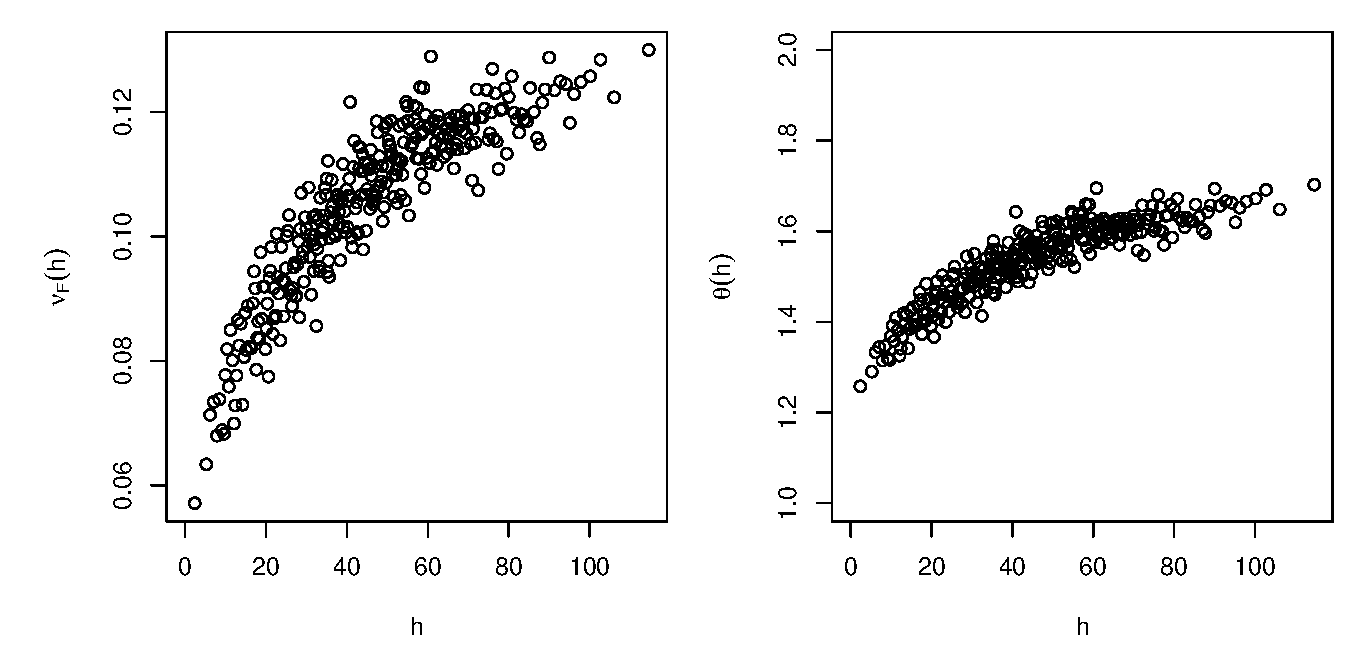
\includegraphics[width=.75\textwidth]{Figures/fmadogramBinned}}
    \caption{Use of the \texttt{fmadogram} function to assess the spatial dependence.}
    \label{fig:fmadogram}
  \end{figure}
  %%%\onslide{4}{\advice{Always think about what should be your spatial coordinates}}
\end{wideslide}

\begin{wideslide}[toc=]{Extremal concurrence probabilities: the \texttt{concprob} function}
  \begin{itemize}
  \item Run the file \texttt{fmadogram.R}. You should get the figure
    below. \textcolor{blue}{Any questions?}
  \item<2-> No? What's wrong?
  \item<3-> You can also use a binned version with \texttt{n.bins =
      300}\ldots
  \end{itemize}
  \begin{figure}
    \centering
    \onslide*{1-2}{\includegraphics[width=.75\textwidth]{Figures/fmadogram}}
    \onslide*{3-}{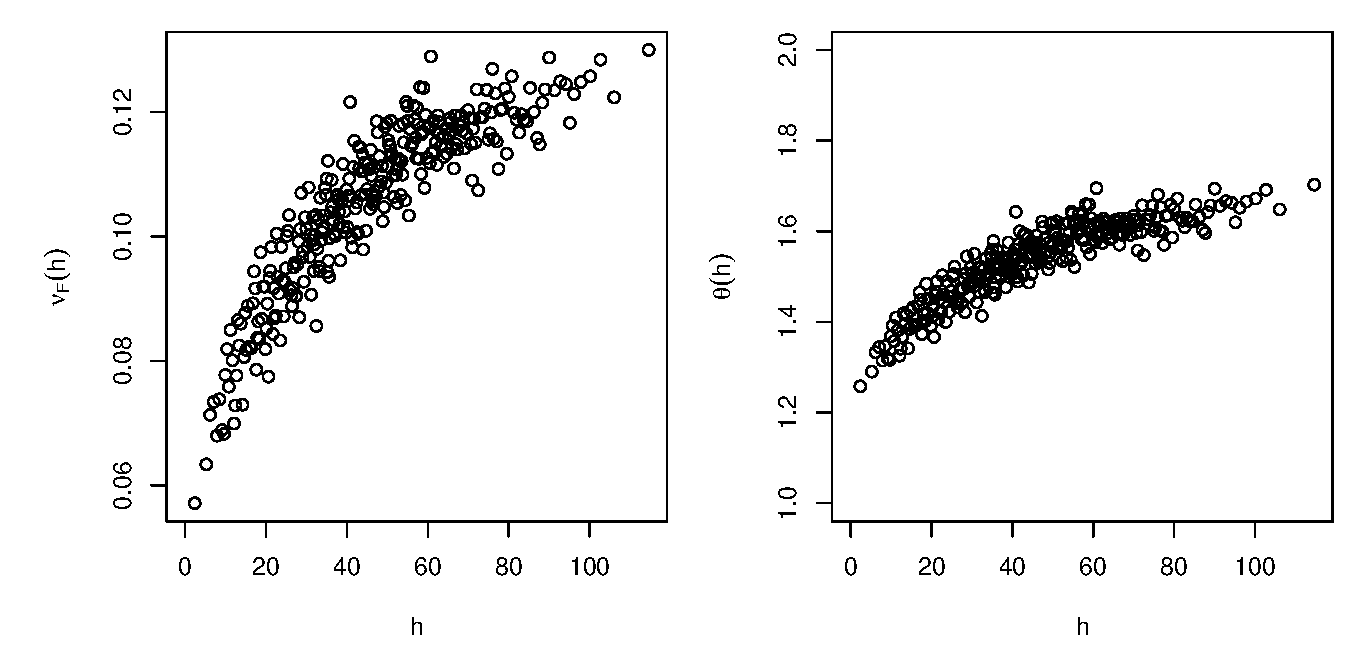
\includegraphics[width=.75\textwidth]{Figures/fmadogramBinned}}
    \caption{Use of the \texttt{fmadogram} function to assess the spatial dependence.}
    \label{fig:fmadogram}
  \end{figure}
  %%%\onslide{4}{\advice{Always think about what should be your spatial coordinates}}
\end{wideslide}



\begin{wideslide}[toc=Spatial trends]{Spatial trends}
  %\vspace*{-1.5em}
  \begin{itemize}
  \item We can do a \textcolor{blue}{symbol plot} but the package
    doesn't have (yet?) a function for this---mainly because it's
    application specific.
  \item Examples at \texttt{SpatialTrends.R} and
    \texttt{SpatialTrends2.R}
  \end{itemize}
  \pause
  \begin{figure}
    \centering
    \onslide*{2}{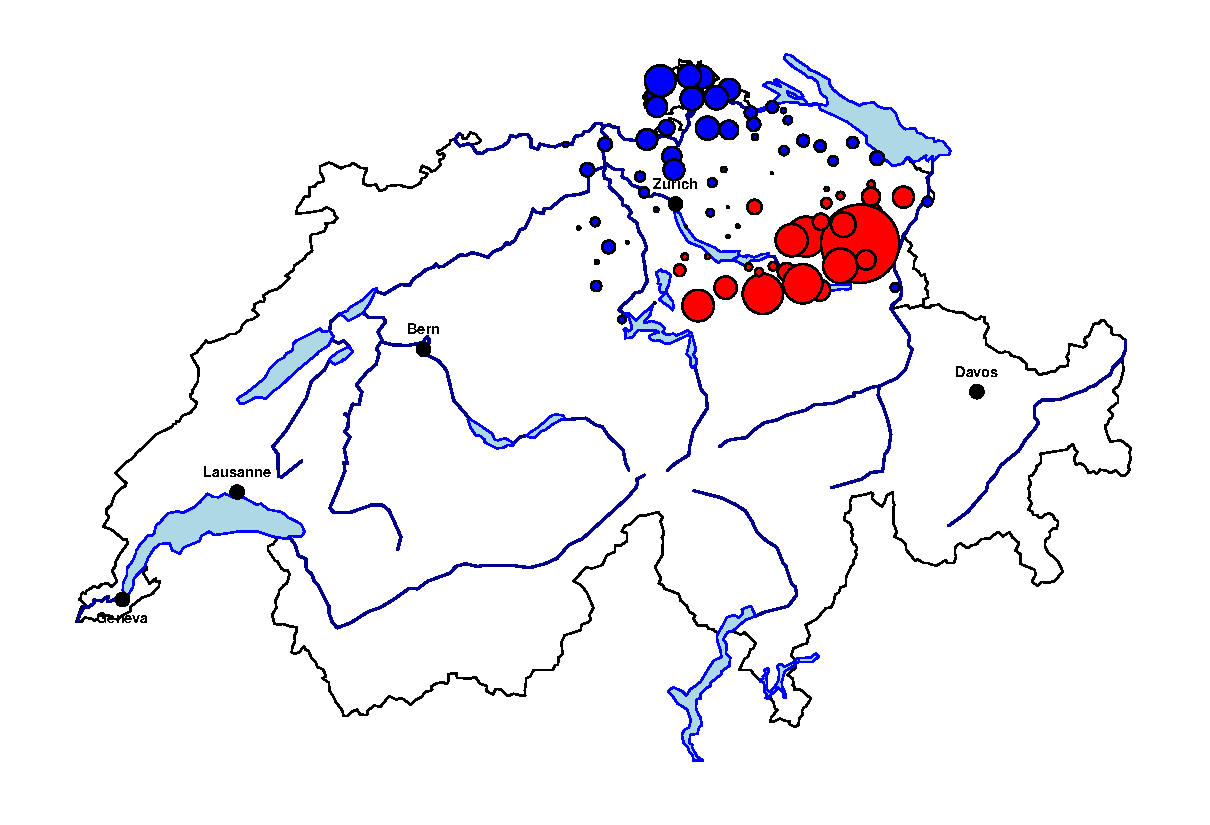
\includegraphics[width=0.5\textwidth]{Figures/symbolPlot}}
    \onslide*{3-}{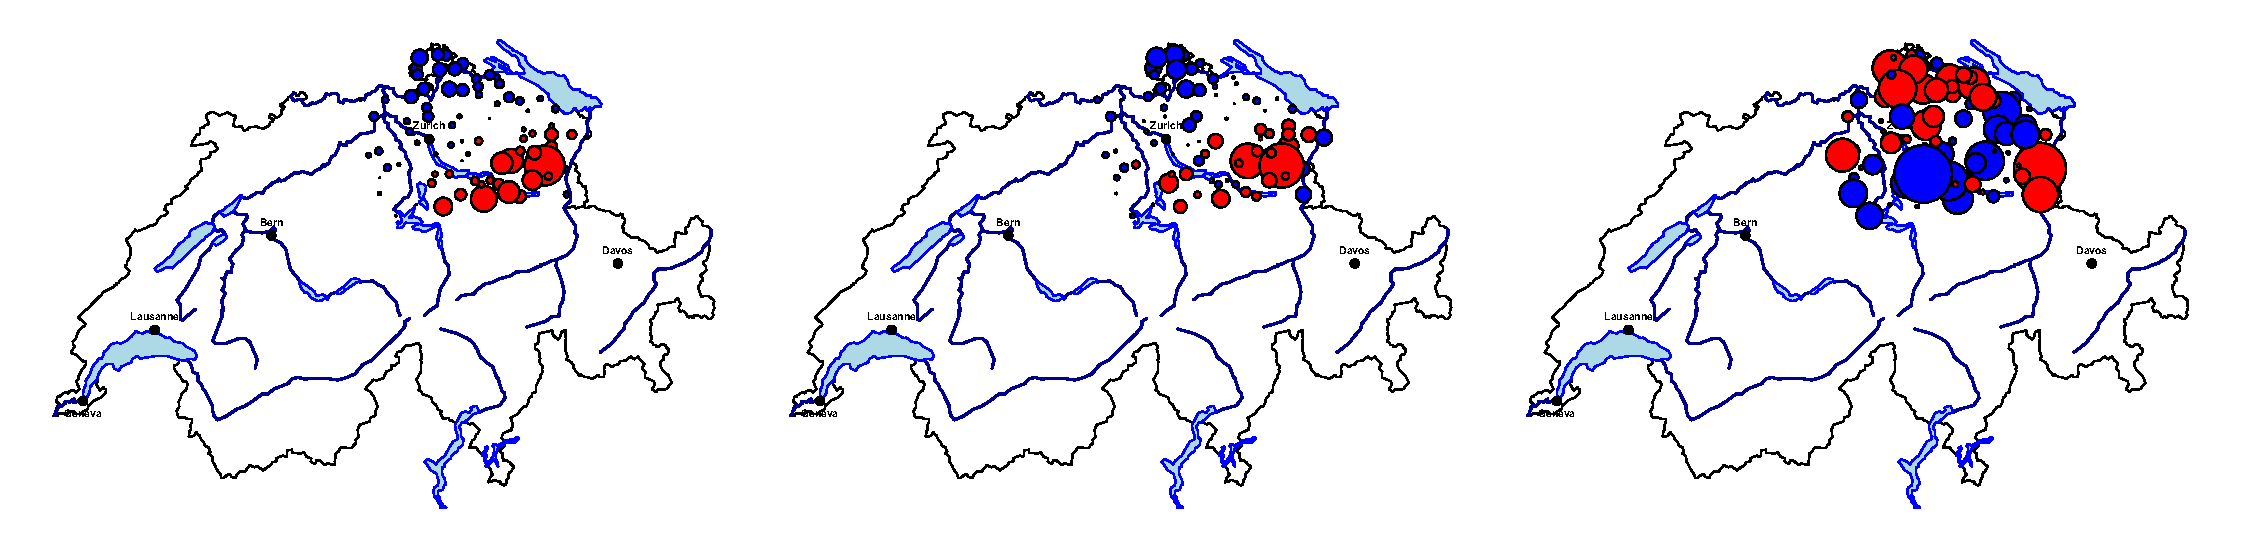
\includegraphics[width=\textwidth]{Figures/symbolPlot2}}
    \caption{Symbol plot for the swiss precipitation data.}
  \end{figure}
  \onslide*{4-}{\advice{When exporting figures into eps/pdf, always
      pay attention to the aspect ratio.}}
\end{wideslide}

\begin{slide}[toc=Debrief \#1]{What we have learned so far (apart from
    using \texttt{SpatialExtremes})}
  \begin{itemize}
  \item The data exhibit some \textcolor{blue}{spatial
      dependence}. The extremal coefficient is around 1.7 for a
    separation lag of 100km---extremes are still not independent but
    close to.
  \item There's a clear \textcolor{blue}{north-west / south-east
      gradient} in the intensities of rainfall storms.
  \item In conclusion it makes sense to use max-stable models whose
    \textcolor{blue}{marginal parameters are not constant across
      space}.
  \item More specifically, we have
    \begin{itemize}
    \item a clear north-west / south-east gradient for the location
      and scale parameters;
    \item no clear pattern for the shape parameter.
    \end{itemize}
  \end{itemize}
\end{slide}

\begin{slide}{Homework}
  \begin{itemize}
  \item Have a look at the temperature and the wind gust data;
  \item Do a descriptive analysis for these two data sets.
  \end{itemize}
\end{slide}


\message{ !name(showv2.tex) !offset(601) }

\end{document}

%%% Local Variables:
%%% mode: latex
%%% TeX-master: t
%%% End:
